\documentclass[tikz,border=4pt]{standalone}
\begin{document}
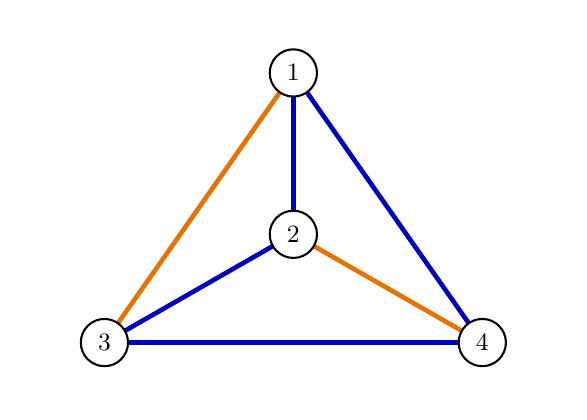
\begin{tikzpicture}[x=0.025cm,y=-0.025cm]
\path[use as bounding box] (0,0) rectangle (270,185);
\path[draw=orange!90!black,fill=none,line width=1.68pt,line join=round] (135,23) -- (39,160);
\path[draw=orange!90!black,fill=none,line width=1.68pt,line join=round] (135,105) -- (231,160);
\path[draw=blue!75!black,fill=none,line width=1.68pt,line join=round] (135,23) -- (135,105);
\path[draw=blue!75!black,fill=none,line width=1.68pt,line join=round] (135,23) -- (231,160);
\path[draw=blue!75!black,fill=none,line width=1.68pt,line join=round] (135,105) -- (39,160);
\path[draw=blue!75!black,fill=none,line width=1.68pt,line join=round] (39,160) -- (231,160);
\path[draw=black,fill=white,line width=.75pt] (135,23) circle[radius=0.3cm];
\node[font=\small,inner sep=0pt] at (135,23) {$1$};
\path[draw=black,fill=white,line width=.75pt] (135,105) circle[radius=0.3cm];
\node[font=\small,inner sep=0pt] at (135,105) {$2$};
\path[draw=black,fill=white,line width=.75pt] (39,160) circle[radius=0.3cm];
\node[font=\small,inner sep=0pt] at (39,160) {$3$};
\path[draw=black,fill=white,line width=.75pt] (231,160) circle[radius=0.3cm];
\node[font=\small,inner sep=0pt] at (231,160) {$4$};
\end{tikzpicture}
\end{document}
